\documentclass[
    12pt,
    a4paper,
    oneside,
    chapter=TITLE,
    section=TITLE,
    subsection=TITLE,
    subsubsection=TITLE,
    english,
    french,
    spanish,
    brazil,
    ]{abntex2}

\usepackage{lmodern}
\usepackage[T1]{fontenc}
\usepackage[utf8]{inputenc}
\usepackage{indentfirst}
\usepackage{color}
\usepackage{graphicx}
\usepackage{microtype}
\usepackage[brazilian,hyperpageref]{backref}
\usepackage[alf]{abntex2cite}

\usepackage{listings}

\renewcommand{\backrefpagesname}{Citado na(s) página(s):~}
\renewcommand{\backref}{}
\renewcommand*{\backrefalt}[4]{
    \ifcase #1
        Nenhuma citação no texto.
    \or
        Citado na página #2.
    \else
        Citado #1 vezes nas páginas #2.
    \fi}

\titulo{PJW HASH FUNCTION}
\autor{DDLS}
\local{Campina Grande}
\data{\today}
\instituicao{
  \textbf{Statement of Work}
  \par
  Instituto Federal de Educação, Ciência e Tecnologia da Paraíba
  }
\tipotrabalho{Projeto de Pesquisa}
\preambulo{Especificação de projeto feito com objetivo de apresentar e auxiliar o desenvolvimento do mesmo, apresentado à comunidade do IFPB}

\definecolor{blue}{RGB}{41,5,195}
\makeatletter
\hypersetup{
        %pagebackref=true,
        pdftitle={\@title}, 
        pdfauthor={\@author},
        pdfsubject={\imprimirpreambulo},
        pdfcreator={LaTeX with abnTeX2},
        pdfkeywords={abnt}{latex}{abntex}{abntex2}{projeto de pesquisa}, 
        colorlinks=false,               
        linkcolor=blue,             
        citecolor=blue,             
        filecolor=magenta,          
        urlcolor=blue,
        bookmarksdepth=4
}
\makeatother

\setlength{\parindent}{1.3cm}
\setlength{\parskip}{0.2cm}

\makeindex

\lstset{
  language=C++,
  basicstyle=\ttfamily\small, 
  keywordstyle=\color{blue}, 
  stringstyle=\color{verde}, 
  commentstyle=\color{red}, 
  extendedchars=true, 
  showspaces=false, 
  showstringspaces=false, 
  numbers=left,
  numberstyle=\tiny,
  breaklines=true, 
  breakautoindent=true, 
  captionpos=b,
  xleftmargin=0pt,
}

\begin{document}

\selectlanguage{brazil}
\frenchspacing 
\imprimircapa
\imprimirfolhaderosto

\pdfbookmark[0]{\contentsname}{toc}
\tableofcontents*
\cleardoublepage

\textual

\chapter{Problema}
Os algoritmos de hash foram uma forma que se encontrou para resumir uma certa quantidade de dados em alguns bits, existem várias formas de se desenvolver um desses algoritmos uma das mais simples é o PJW que transforma as palavras de entrada em saídas de 32 bits. Com base nessas duas implementações abaixo desenvolva um IP Core que calcule a palavra hash da mesma maneira.

\par
Implementação 1:
\begin{lstlisting}
unsigned long ElfHash ( const unsigned char *s )
{
    unsigned long   h = 0, high;
    while ( *s )
    {
        h = ( h << 4 ) + *s++;
        if ( high = h & 0xF0000000 )
            h ^= high >> 24;
        h &= ~high;
    }
    return h;
}
\end{lstlisting}

\par
Implementação 2:
\begin{lstlisting}
static unsigned int ELFHash(string str) {
    unsigned int hash = 0;
    unsigned int x = 0;
    unsigned int i = 0;
    unsigned int len = str.length();

    for (i = 0; i < len; i++)
    {
        hash = (hash << 4) + (str[i]);
        if ((x = hash & 0xF0000000) != 0)
        {
            hash ^= (x >> 24);
        }
        hash &= ~x;
    }
    return hash;
}
\end{lstlisting}

\chapter{Interface}

A interface de comunicação do seu sistema deve atender os seguintes requisitos da \autoref{tabela-interface}:

\begin{table}[htb]
\IBGEtab{
  \caption{Especificação de Dados}
  \label{tabela-interface}
}{
  \begin{tabular}{ccc}
  \toprule
   Nome & Tipo & Tamanho em bits \\
  \midrule \midrule
   Valid & Entrada & 1 \\
  \midrule 
   DataIn & Entrada & 32 \\
  \midrule 
   Ready & Saída & 1 \\
  \midrule 
   DataOut & Saída & 32 \\
  \bottomrule
\end{tabular}
}{
  \fonte{Produzido pelos autores.}%
  \nota{Ready será levado para 1 quando o IP estiver pronto para entrada ou saída de dados.}
  \nota{Valid só será ativado quando o ready estiver levantado e servirá para a entrada de dados.}
  \nota{DataIn só será gravado quando o Valid e o Ready estiverem ativos.}
  }
\end{table}

Na \autoref{fig-maquina-estados} você pode analisar a maquina de estados do sistema.
\par
\begin{figure}[htb]
    \caption{\label{fig-maquina-estados}Maquina de Estados da Interface}
    \begin{center}
        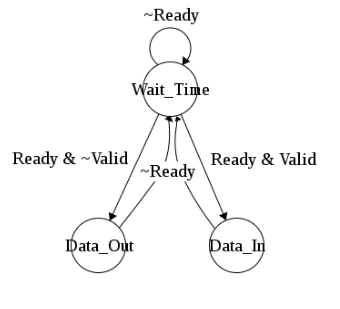
\includegraphics[scale=0.8]{imgs/maquina-estados.png}
    \end{center}
    \legend{Fonte: Produzido pelos autores.}
\end{figure}


\chapter{Estimulos}
\section{Entrada}
O primeiro dado que deverá entrar é um número n, após isso haverá a entrada de n palavras k.
\par
Onde 0 < n < 8

\section{Saída}
A saída deverá ser mostrada apenas quando o hash houver sido calculado e deve sair junto com a subida do ready após 1+n entradas de dados.

\section{Caso Base}
Na \autoref{fig-caso-PJW} temos um exemplo de como deve seu IP deve responder com os respectivos estímulos.

\begin{figure}[htb]
    \caption{\label{fig-caso-PJW}Caso Base do PJW Hash}
    \begin{center}
        \advance\leftskip-3cm
        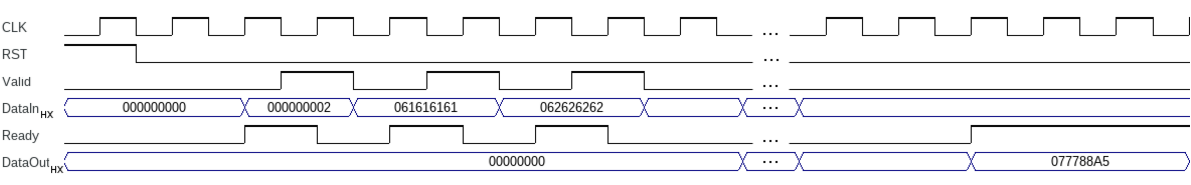
\includegraphics[width=\paperwidth]{imgs/caso-PJW.png}
    \end{center}
    \legend{Fonte: Produzido pelos autores.}
\end{figure}

\end{document}